\let\negmedspace\undefined
\let\negthickspace\undefined
\documentclass[journal]{IEEEtran}
\usepackage[a5paper, margin=10mm, onecolumn]{geometry}
\usepackage{lmodern} 
\usepackage{tfrupee} 

\setlength{\headheight}{1cm} % Set the height of the header box
\setlength{\headsep}{0mm}     % Set the distance between the header box and the top of the text

\usepackage{gvv-book}
\usepackage{gvv}
\usepackage{cite}
\usepackage{amsmath,amssymb,amsfonts,amsthm}
\usepackage{algorithmic}
\usepackage{graphicx}
\usepackage{textcomp}
\usepackage{xcolor}
\usepackage{txfonts}
\usepackage{listings}
\usepackage{enumitem}
\usepackage{mathtools}
\usepackage{gensymb}
\usepackage{comment}
\usepackage[breaklinks=true]{hyperref}
\usepackage{tkz-euclide} 
\usepackage{listings}                                      
\def\inputGnumericTable{}                                 
\usepackage[latin1]{inputenc}                                
\usepackage{color}                                            
\usepackage{array}                                            
\usepackage{longtable}
\usepackage{multicol}
\usepackage{calc}                                             
\usepackage{multirow}                                         
\usepackage{hhline}                                           
\usepackage{ifthen}                                           
\usepackage{lscape}
\begin{document}

\bibliographystyle{IEEEtran}
\vspace{3cm}

\title{8.4.34}
\author {EE25BTECH11031 - Sai Sreevallabh}
% \maketitle
% \newpage
% \bigskip
{\let\newpage\relax\maketitle}

\renewcommand{\thefigure}{\theenumi}
\renewcommand{\thetable}{\theenumi}
\setlength{\intextsep}{10pt} % Space between text and floats


\numberwithin{equation}{enumi}
\numberwithin{figure}{enumi}
\renewcommand{\thetable}{\theenumi}

\textbf{Question: }\\

Let $\brak{x,y}$, be any point on the parabola $y^2 = 4x$. Let $\vec{P}$ be the point that divides the line segment from $\brak{0,0}$ to $\brak{x,y}$ in the ration 1:3. Then the locus of $\vec{P}$ is.
\begin{enumerate}
\begin{multicols}{4}
    \item $x^2 = y$
    \item $y^2 = 2x$
    \item $y^2 = x$
    \item $x^2 = 2y$
\end{multicols}
\end{enumerate}

\textbf{Solution}\\

Given points can be taken to be
\begin{align}
    \vec{O} = \myvec{0\\0} \ \text{and} \ \vec{Q} = \myvec{x\\y}
\end{align}

Point $\vec{P} = \myvec{x_p\\y_p}$ divides the line segment $\vec{P-O}$ in the ratio 1:3. so
\begin{align}
    \vec{P} = \frac{3\vec{O}+\vec{Q}}{3+1}\\
    \implies \myvec{x_p\\y_p} = \frac{1}{4}\myvec{x\\y}
\end{align}

So, 
\begin{align}
    x = 4x_p \ \ \text{and} \ \ y = 4y_p
\end{align}

Substituting the above in the equation in the parabola $y^2 = 4x$.
\begin{align}
    y_p^2 = x_p
\end{align}

Therefore, the locus of the point $\vec{P}$ is the parabola $y^2 = x$. 

\begin{figure}
    \centering
    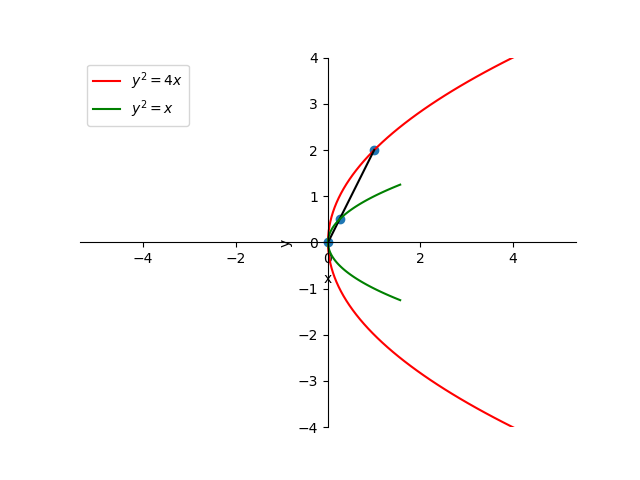
\includegraphics[width=1\columnwidth]{Figs/plot(py+C).png}
\end{figure}

\end{document}
